%% 该模板修改自《计算机学报》latex 模板
%% 主要是将双栏改成单栏，去掉了部分计算机学报标识；
%% 源文件自：https://www.overleaf.com/latex/templates/latextemplet-cjc-xelatex/ybmmymncrrmw
%% 
%%
%% This is file `CjC_template_tex.tex',
%% is modified by Zhi Wang (zhiwang@ieee.org) based on the template 
%% provided by Chinese Journal of Computers (http://cjc.ict.ac.cn/).
%%
%% This version is capable with Overleaf (XeLaTeX).
%%
%% Update date: 2023/03/10
%% -------------------------------------------------------------------
%% Copyright (C) 2016--2023 
%% This file may be distributed and/or modified under the
%% conditions of the LaTeX Project Public License, either version 1.3c
%% of this license or (at your option) any later version.
%% The latest version of this license is in
%%    https://www.latex-project.org/lppl.txt
%% and version 1.3c or later is part of all distributions of LaTeX
%% version 2008 or later.
%% -------------------------------------------------------------------
\newcommand{\todoc}[2]{{\textcolor{#1}{\textbf{#2}}}}
\newcommand{\todoblue}[1]{\todoc{blue}{\textbf{[[#1]]}}}
\documentclass[10.5pt,compsoc,UTF8]{cjc}
% \usepackage{algorithmic}
\usepackage{algorithm} % 展示算法伪代码
\usepackage{CTEX}
\usepackage{subcaption}
\usepackage{graphicx}
\usepackage{footmisc}
% \usepackage{subfigure}
\usepackage{url}
\usepackage{multirow}
\usepackage{multicol}
\usepackage[noadjust]{cite}
\usepackage{amsmath,amsthm}
\usepackage{amssymb,amsfonts}
\usepackage{booktabs}
\usepackage{color}
% \usepackage{ccaption}
\usepackage{booktabs}
\usepackage{float}
\usepackage{fancyhdr}
% \usepackage{caption}
\usepackage{xcolor,stfloats}
\usepackage{comment}
\setcounter{page}{1}
\graphicspath{{figures/}}
\usepackage{cuted}%flushend,
% \usepackage{captionhack}
\usepackage{epstopdf}
\usepackage{gbt7714}
\usepackage{setspace}
\usepackage{listings}
\usepackage{hyperref}
\usepackage{minted}
\usepackage{tocloft} % 用于调整目录格式
% \usepackage[linesnumbered,ruled,vlined]{algorithm2e}
% \usepackage{algorithm}
% \usepackage{algorithmic}

\usepackage{algpseudocode}


%===============================%

% 设置 listings 包的一些选项
\lstset{
    basicstyle=\ttfamily, % 字体样式
    showstringspaces=false, % 不显示字符串中的空格
    breaklines=true, % 自动换行长行
    tabsize=2, % tab 的宽度
    frame=single, % 添加单边框
    backgroundcolor=\color{lightgray}, % 设置背景颜色
    xleftmargin=10pt, % 左边距
    xrightmargin=10pt, % 右边距
    aboveskip=\baselineskip, % 上方间距
    belowskip=\baselineskip % 下方间距
}

\captionsetup[figure]{name=图}
\renewcommand{\lstlistingname}{代码}
\headevenname{\leftmark}%
\headoddname{\rightmark}%


% 自定义目录标题格式
\renewcommand{\cfttoctitlefont}{\Huge} % 目录标题居中并加大字体
\renewcommand{\cftlottitlefont}{\Huge} % 表格目录标题居中并加大字体
\renewcommand{\cftloftitlefont}{\Huge} % 插图目录标题居中并加大字体

% 自定义目录标题与内容的距离
\renewcommand{\cftbeforetoctitleskip}{0.5cm} % 目录标题与目录内容之间的距离
\renewcommand{\cftbeforelottitleskip}{0.5cm} % 表格目录标题与目录内容之间的距离
\renewcommand{\cftbeforeloftitleskip}{0.5cm} % 插图目录标题与目录内容之间的距离

% 调整目录条目间距
\renewcommand{\cftaftertoctitleskip}{2cm}
\renewcommand{\cftafterlottitleskip}{2cm}
\renewcommand{\cftafterloftitleskip}{2cm}


%footnote use of *
\renewcommand{\thefootnote}{\fnsymbol{footnote}}
\setcounter{footnote}{0}
\renewcommand\footnotelayout{\zihao{5-}}

\newtheoremstyle{mystyle}{0pt}{0pt}{\normalfont}{1em}{\bf}{}{1em}{}
\theoremstyle{mystyle}
\renewcommand\figurename{figure~}
% \renewcommand{\thesubfigure}{(\alph{subfigure})}
\newcommand{\upcite}[1]{\textsuperscript{\cite{#1}}}
\renewcommand{\labelenumi}{(\arabic{enumi})}
\newcommand{\tabincell}[2]{\begin{tabular}{@{}#1@{}}#2\end{tabular}}
\newcommand{\abc}{\color{white}\vrule width 2pt}
\renewcommand{\bibsection}{}
\makeatletter
\renewcommand{\@biblabel}[1]{[#1]\hfill}
\makeatother
\setlength\parindent{2em}
\setlength{\textwidth}{15.2cm}  % 设置正文宽度为15.2厘米
\setlength{\oddsidemargin}{0.4cm}  % 增加奇数页的左边距
\setlength{\evensidemargin}{0.4cm} % 增加偶数页的左边距
%\renewcommand{\hth}{\begin{CJK*}{UTF8}{gbsn}}
%\renewcommand{\htss}{\begin{CJK*}{UTF8}{gbsn}}


\begin{document}

\hyphenpenalty=50000
\makeatletter
\newcommand\mysmall{\@setfontsize\mysmall{7}{9.5}}
\newenvironment{tablehere}
  {\def\@captype{table}}

\let\temp\footnote
\renewcommand \footnote[1]{\temp{\zihao{-5}#1}}


\thispagestyle{plain}%
\thispagestyle{empty}%
\pagestyle{CjCheadings}

% \begin{table*}[!t]
\vspace {-13mm}


\onecolumn
\zihao{5-}\noindent  \hfill RCPTA 两阶段静态分析与 Cast Site 诊断设计说明文档 \hfill 2026 年 7 月\\
\noindent\rule[0.25\baselineskip]{\textwidth}{1pt}

% \onecolumn
% \zihao{5-}\noindent 第??卷\quad 第?期 \hfill 计\quad 算\quad 机\quad 学\quad 报\hfill Vol. ??  No. ?\\
% \zihao{5-}
% 20??年?月 \hfill CHINESE JOURNAL OF COMPUTERS \hfill ???. 20??\\ 
% \noindent\rule[0.25\baselineskip]{\textwidth}{1pt}

{
\centering
\vspace {11mm}
{
    \zihao{2} \heiti 南京大学-小米软件部\\\vspace{1cm}
    \zihao{4} \heiti RCPTA 两阶段静态分析与 Cast Site 诊断工具设计说明文档
}

\vskip 5mm

{ }

% \footnote{\noindent \zihao{6} 
% % 收稿日期：\quad \quad -\quad -\quad ；最终修改稿收到日期：\quad \quad -\quad -\quad .*投稿时不填写此项*. 本课题得到… …基金中文完整名称(No.项目号)、… …基金中文完整名称(No.项目号)、… … 基金中文完整名称(No.项目号)资助.
% \textsf{作者名1}，学号，学位(或目前学历),主要研究领域为*****、****. E-mail: **************.\textsf{作者名2}，学号，学位(或目前学历),主要研究领域为*****、****. E-mail: **************. \textsf{作者名3}，学号，学位(或目前学历),主要研究领域为*****、****. E-mail: **************.}

\vspace {5mm}

\textbf{\zihao{4}{\heiti 南京大学可信软件实验室}}

% \zihao{5}{$^{2)}$(单位全名 部门(系)全名, 市(或直辖市) 国家名 邮政编码)*中英文单位名称、作者姓名须一致*}

% \zihao{5}{$^{3)}$(单位全名 部门(系)全名, 市(或直辖市) 国家名 邮政编码)}

% \zihao{6}{\textsf{论文定稿后，作者署名、单位无特殊情况不能变更。若变更，须提交签章申请，国家为中国可以不写，省会城市不写省名，其他国家必须写国家名。}}
}

\vskip 5mm

% \zihao{5}{
% \setlength{\baselineskip}{16pt}\selectfont{
% \noindent {\heiti 摘\quad 要\quad }
% *中文摘要内容置于此处(英文摘要中要有这些内容)，字体为5号宋体。摘要贡献部分，要有数据支持，不要出现``...大大提高''、``...显著改善''等描述，正确的描述是``比{\ldots}提高X{\%}''、``在{\ldots}上改善X{\%}''。
% \par}}
% \vspace {5mm}

% \zihao{5}{\noindent
% {\heiti 关键词 \quad }{*关键词（中文关键字与英文关键字对应且一致，应有5-7个关键词)；关键词；关键词*  }
% }
% \zihao{5-}{\heiti 中图法分类号\quad } TP\rm{\quad \quad \quad     }
% {\heiti DOI号:\quad } *投稿时不提供DOI号


\vskip 7mm

% \begin{center}
% \zihao{3}{ \heiti Title *（中英文题目一致)字体为4号Times New Roman,加粗* Title}\\
% \vspace {5mm}
% \zihao{5}{ NAME Name-Name$^{1)}$ NAME Name$^{2)}$ NAME Name-Name$^{3)}$ *字体为5号Times new Roman*Name}\\
% \vspace {2mm}
% \zihao{5-}{{$^{1)}$(Department of ****, University, City ZipCode, China) *字体为小5号Times new Roman* Depart.Correspond}}

% \zihao{5-}{{$^{2)}$(Department of ****, University, City ZipCode)*中国不写国家名*}}

% \zihao{5-}{{$^{3)}$(Department of ****, University, City ZipCode, country)*外国写国家名*}}

% \end{center}

% \zihao{5}{
% \setlength{\baselineskip}{18pt}\selectfont{
% {\bf Abstract}\quad (\textbf{500英文单词，内容包含中文摘要的内容}).
% 字体为Times new Roman,字号5号* 
% \zihao{5}{\noindent Do not modify the amount of space before and after the artworks. One- or two-column format artworks are preferred. and Tables, create a new break line and paste the resized artworks where desired. Do not modify the amount of space before and after the artworks. One- or two-column format artworks are preferred. All Schemes, Equations, Figures, and Tables should be mentioned in the text consecutively and numbered with Arabic numerals, and appear below where they are mentioned for the first time in the main text. To insert Schemes, Equations, Figures, and Tables, create a new break line and paste the resized artworks where desired. Do not modify the amount of space before and after the artworks. One- or two-column format artworks are preferred.Do not modify the amount of space before and after the artworks. One- or two-column format artworks are preferred. and Tables, create a new break line and paste the resized artworks where desired. %Do not modify the amount of space before and after the artworks. One- or two-column format artworks are preferred. All Schemes, Equations, Figures, and Tables should be mentioned in the text consecutively and numbered with Arabic numerals, and appear below where they are mentioned for the first time in the main text.
% \par}}
% \vspace {5mm}

% {{\bf Keywords}\quad 中文关键字与英文关键字对应且一致，\textbf{不要用英文缩写});
% key word; key word; key word* *字体为5号Times new Roman * Key words\par}}


%%%%%%%%%%%%%%%%%%%%%%%%%%%%%%%%%%%%%%
\vskip 10mm
\newpage
\markboth{目录}{目录}
\renewcommand{\contentsname}{\heiti 目录}
\tableofcontents
\newpage
% \markboth{表格目录}{表格目录}
% \renewcommand{\listtablename}{\heiti 表格目录}
% \listoftables
% \newpage
% \markboth{插图目录}{插图目录}
% \renewcommand{\listfigurename}{\heiti 插图目录}
% \listoffigures
% \begin{multicols}{1}

\newcommand{\zcy}[1]{\textcolor{red}{ZCY:#1}}




%%%%%%%%%%%%%%%%%%%%%%%%%%%%%%%%%%%%%%%%%%
%%%%%%%%%%%%%%%%%%%%%%%%%%%%%%%%%%%%%%%%%%

\newpage
\doublespacing
\thispagestyle{empty}

{\raggedright
\zihao{1}
\section{\heiti\centering 项目设计}}
\zihao{4-}

\subsection{项目总体能力介绍}

本项目旨在构建面向 Rust 面向对象风格 DSL 的静态分析框架 RCPTA（Rust Class Pointer Type Analysis），在 RUPTA 的 Rust MIR 指针分析基础上，为采用 class、extends、interface、mixin 与引用计数对象包装的 Rust DSL 程序提供源码级可解释的对象流、类型流与 cast site 诊断结果。项目经历两个阶段：第一阶段围绕旧 Rust class DSL 建立类级指针分析基础能力，验证 ClassPAG、Class PTS、Class Call Graph、动态类型集合和 cast risk detection 在 animal、shape、vehicle 与综合层次测试套件中的可用性；第二阶段在此基础上面向新的 Lite Class DSL 和 cast erase 需求，进一步强化 wrapper/container 摘要建模，构造专门的 \texttt{cast\_risk\_matrix} 数据集，并完成 checked cast site 的 safe/may-unsafe/must-unsafe/unknown 分类闭环。

RCPTA 的核心输出不只是传统 points-to 集合，而是一组可审计的分析产物：\texttt{class\_pag.txt} 描述类级指针赋值图，\texttt{class\_pts.txt} 描述类级指向集，\texttt{class\_cg.txt} 描述类级调用图，\texttt{type-info.txt} 将 points-to 对象集合投影为动态类型集合，\texttt{inheritance\_graph.txt} 给出 class/interface/mixin 类型关系，\texttt{cast\_safety.log} 对源码级 checked cast 输出诊断。通过这些产物，工具能够从 MIR 层复杂展开中恢复开发者关心的“某个类对象可能流向哪里”“某个 receiver 可能有哪些动态类型”“某个 downcast 是否可被静态证明安全”等源码级问题。

截至第二阶段收尾，旧 DSL 测试套件的 51 个入口已经能够完成分析并生成完整产物，其中包括此前存在栈溢出问题的 vehicle 属性测试入口；新的 Lite Class DSL 部分除专门构造的 \texttt{cast\_risk\_matrix} 外，还对 \texttt{animal\_hierarchy}、\texttt{shape\_hierarchy} 与 \texttt{vehicle\_hierarchy} 三套原始 DSL 测试套件进行了 RCPTA 兼容性分析。最终 cast risk matrix 覆盖 90 个高价值 cast 场景，诊断统计为 \textbf{43 个 safe、40 个 may-unsafe、7 个 must-unsafe、0 个 unknown}，且没有空 points-to 导致的 cast 源未知结果；按源码真实语义审计，三分类 exact accuracy 为 \textbf{88/90 = 97.78\%}，剩余 2 个错误均为真实安全场景被保守报为 may-unsafe 的假阳性，未发现真实不安全场景被误判为 safe 的假阴性。

\subsection{项目背景}

静态分析旨在不执行程序的前提下，对程序可能状态进行保守抽象。指针分析是静态分析的重要基础，它决定了对象流、别名关系、调用图构建、动态类型范围估计以及类型转换安全性判断的精度。对于采用面向对象风格的 Rust DSL 程序而言，普通 MIR 层指针分析结果通常表现为局部变量、临时引用、投影路径、标准库调用和宏展开后的 runtime helper，难以直接对应源码层的类、对象、字段、方法、接口、多态调用和 checked cast。

旧 Rust class DSL 和新的 Lite Class DSL 都通过 Rust 宏与类型系统模拟 OO 语义。源码层中，程序员会书写 \texttt{Dog::new()}、\texttt{CRc<Animal>}、\texttt{CRc<Runnable>}、\texttt{downcast\_rc::<Dog>()}、\texttt{downcast\_ref::<Tagged>()} 等类级操作；但编译后，这些操作会展开为复杂的泛型、trait、引用、\texttt{Option}/\texttt{Result} 和容器 API。若没有专门的类级抽象，分析器很容易出现两类问题：一是有效对象流在 MIR 临时路径之间断开，导致 points-to 为空；二是无关对象被过度合并，导致本应 safe 的 cast 被误报为 may-unsafe。

因此，RCPTA 的目标是建立一层面向 DSL class 语义的中间抽象。第一阶段解决“能否从 MIR 中恢复类级对象流和调用关系”的问题；第二阶段进一步解决“能否在常见 wrapper/container/API 形态下稳定诊断 cast site”的问题。最终，RCPTA 要为 cast erase / checked cast 优化提供静态证据：safe cast 可作为优化候选，must-unsafe cast 表示必然失败路径，may-unsafe cast 表示需要保留运行时检查或进一步路径敏感分析，unknown 则提示上游建模仍存在缺口。

\subsection{总体设计方案}

项目采用分层架构：底层复用 RUPTA 对 Rust MIR 的解析、函数遍历和基础指针分析设施；中间层由 RCPTA 将 DSL 类引用相关 MIR 操作抽象为 ClassPtr、ClassObj 与 ClassPAG；上层基于 ClassPTS 计算动态类型集合，解析 DSL 类型关系，并执行 cast safety 分类。

在 MIR 遍历阶段，RCPTA 识别类构造、类引用复制、clone、类型转换、字段读写、方法调用、函数参数与返回值传播，并在 ClassPAG 中加入 Alloc、Assign、Cast、Load、Store、CallArg、CallRet 等边。ClassPTS 求解器随后在 ClassPAG 上进行迭代传播，得到每个 ClassPtr 可能指向的 ClassObj 集合。由于每个 ClassObj 都记录其源码级类名，工具可以进一步得到：
\[
    \mathrm{TypeRange}(ptr)=\{\,\mathrm{class\_type}(obj)\mid obj\in \mathrm{PTS}(ptr)\,\}.
\]

对于 cast site，工具同时需要目标类型和类型兼容关系。RCPTA 从 DSL 声明中抽取 \texttt{extends}、\texttt{implements}、\texttt{with}、\texttt{mixin on} 等关系，构建继承/接口/mixin 图，并计算用于判定的闭包关系。普通 class 目标使用继承闭包，interface 目标使用实现闭包，mixin 目标使用 \texttt{with*} 关系。Cast safety classifier 最终比较源动态类型集合和目标类型，输出 \texttt{safe}、\texttt{may-unsafe}、\texttt{must-unsafe} 或边界未知类结果。

%%%%%%%%%%%%%%%%%%%%%%%%%%%%%%%%%%%%%%%%%%
%%%%%%%%%%%%%%%%%%%%%%%%%%%%%%%%%%%%%%%%%%
\newpage
\doublespacing
\thispagestyle{empty}

{\raggedright
\zihao{1}
\section{\heiti\centering 具体设计}}
\zihao{4-}

\subsection{总览}

RCPTA 的总体架构如图~\ref{fig:rcpta-stage2-architecture} 所示。输入为 Rust DSL 程序和指定入口函数，分析器通过 \texttt{cargo-pta} 在编译过程中获取 MIR。构建阶段产生 ClassPAG 与 cast site 记录；求解阶段输出 ClassPTS 与 cast 源快照；结果阶段生成类型集合、继承关系和 cast safety 诊断。

\begin{figure}[H]
    \centering
    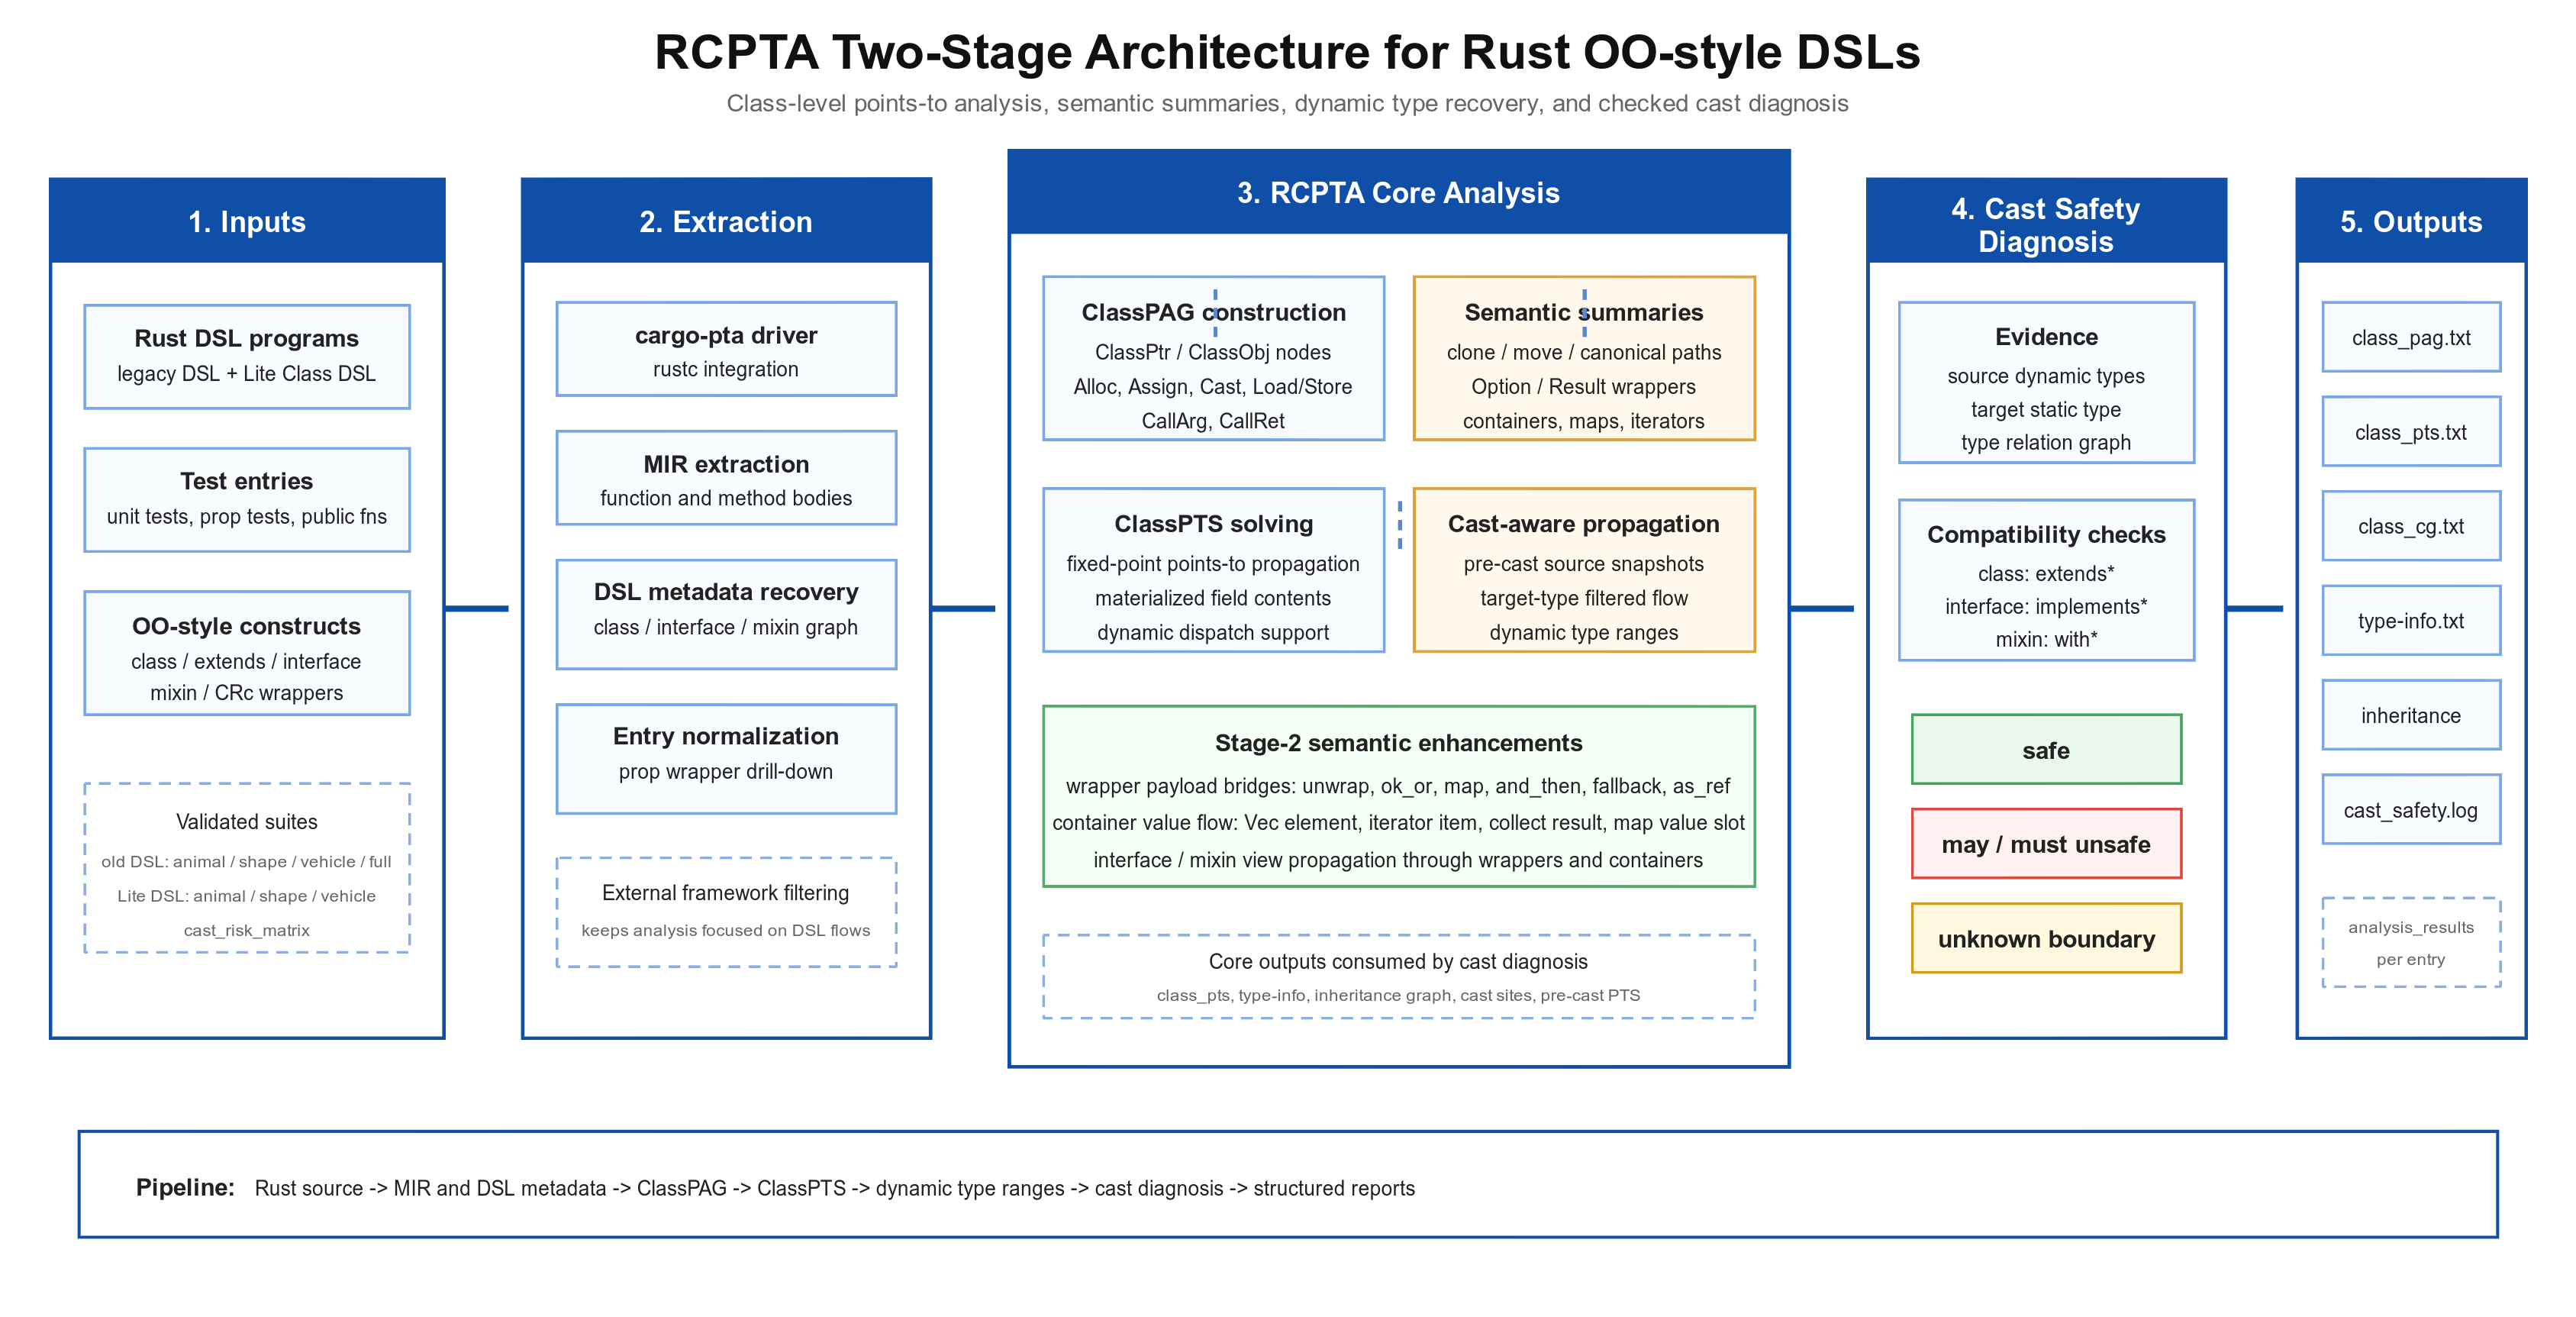
\includegraphics[width=\textwidth]{rcpta_arc_v3.png}
    \caption{RCPTA 类级分析与 cast 诊断总体架构}
    \label{fig:rcpta-stage2-architecture}
\end{figure}

需要强调的是，RCPTA 并不替代底层 MIR 指针分析，而是在其上建立面向 DSL class 的语义层。该语义层的输出应尽量对应源码中的类对象、字段、wrapper payload、容器元素和 cast site，而不是暴露大量标准库或宏展开内部临时状态。

\subsection{类级指针与堆对象}

RCPTA 中的类级指针 ClassPtr 表示“可能持有 DSL 类对象引用”的路径。它既可以对应局部变量、参数和返回值，也可以对应字段、wrapper payload、container element slot、map value slot 或 cast 结果。实现中，ClassPtr 通过字符串 ID 与静态 class type 标识，例如 \texttt{func::local\_1}、\texttt{func::ret}、\texttt{func::local\_5.as\_variant\#0.0} 或 \texttt{func::local\_24.\$elem}。

堆对象 ClassObj 使用分配点抽象。每个源码级类构造调用在 ClassPAG 中对应一个抽象对象，记录对象 ID、动态类名和分配点。分配点由函数和 MIR 位置确定，因此同一代码位置的运行时对象归约为同一个 ClassObj。该堆抽象在本项目目标下是合适的：cast safety 关注动态类型集合，而动态类型集合可以由 ClassObj 的 \texttt{class\_type} 直接投影得到。

\subsection{ClassPAG 边与求解规则}

ClassPAG 的边语义如下：

\begin{enumerate}
    \item \textbf{Alloc}：对象创建，例如 \texttt{Dog::new()} 将目标 ClassPtr 指向一个 \texttt{Dog} ClassObj。
    \item \textbf{Assign}：类引用复制、\texttt{clone()}、wrapper payload 移动、container 元素传播等，不改变对象身份。
    \item \textbf{Cast}：同一对象的类型视图转换或 checked cast。Cast 边传播时按目标类型兼容性过滤对象。
    \item \textbf{Load/Store}：字段读写。Store 将源 points-to 写入 \texttt{content[obj, field]}，Load 从该内容传播到读取结果。
    \item \textbf{CallArg/CallRet}：跨函数传播，将调用方实参传播到被调函数形参，将被调函数返回值传播到调用方接收位置。
\end{enumerate}

ClassPTS 求解采用迭代传播直到不动点。Alloc 初始化 \texttt{pts(ptr)}；Assign、Cast、CallArg、CallRet 传播对象集合；Store/Load 在对象字段层面物化内容。Cast 边除了传播对象，还会记录 cast 前源指针的 points-to 快照 \texttt{cast\_src\_before\_pts}，供后续安全判定使用，避免使用 cast 后结果造成自污染。

\subsection{路径规范化与别名处理}

MIR 中同一个源码级类引用常常会被拆成多个临时路径。例如 \texttt{x.clone()} 可能涉及 \texttt{\&x}、receiver 临时变量、返回临时变量和 move；\texttt{unwrap()} 可能表现为对 \texttt{Option} 或 \texttt{Result} variant payload 的投影；方法调用还会引入 receiver 引用和参数 copy。若 ClassPAG 直接使用这些原始路径，实际对象流会断开。

因此，RCPTA 维护 canonical pointer 与引用基路径映射。引用临时变量会映射回被借用的 base path；copy/move 会维护别名关系；wrapper holder 的 move 会记录原始 holder 路径，使后续 \texttt{unwrap()} 能回到正确的 \texttt{Some.0}/\texttt{Ok.0} payload。构建 Assign、Cast、CallArg 与 clone 边时，分析器优先使用 canonical ClassPtr，从而减少由 MIR 临时变量造成的空 points-to。

\subsection{DSL 类型关系与 cast 判定}

类型关系图从 DSL 声明中抽取节点和边。旧 DSL 阶段主要解析 \texttt{pub class}、\texttt{pub abstract class}、\texttt{pub mixin}、\texttt{extends}、\texttt{implements}、\texttt{with} 与 \texttt{mixin on}；Lite Class DSL 阶段则进一步适配 \texttt{\#[class(extends(...))]}、\texttt{type X = class<...>}、\texttt{interface<...>} 和 \texttt{mixin<...>} 这类声明形态。

Cast safety 判定规则如下。若目标为普通 class，要求源动态类型满足 class subtype，即目标类型本身或其子类；若目标为 interface，要求源动态类型实现该 interface；若目标为 mixin，要求源动态类型显式具有该 mixin 视图。根据满足集合和不满足集合，分类为：

\begin{itemize}
    \item \texttt{safe}：所有源动态类型都满足目标类型；
    \item \texttt{may-unsafe}：部分源动态类型满足，部分不满足；
    \item \texttt{must-unsafe}：所有源动态类型都不满足；
    \item \texttt{boundary-unknown-src} 或 \texttt{boundary-missing-dst-type}：缺少源动态类型或目标类型证据。
\end{itemize}

\subsection{Wrapper 摘要建模}

第二阶段大量精度改进集中在 wrapper payload 建模。RCPTA 将 \texttt{Option::unwrap}、\texttt{Result::unwrap} 建模为 payload 到返回值的 Assign；将 \texttt{Option<Result<...>>} 和 \texttt{Result<Option<...>>} 建模为多级 payload path；将 \texttt{Option::ok\_or} 建模为 \texttt{Some.0} 到 \texttt{Ok.0} 的转换；将 \texttt{map} 与 \texttt{and\_then} 建模为通过闭包参数和闭包返回值传播 payload；将 \texttt{or}、\texttt{or\_else}、\texttt{unwrap\_or\_else} 等 fallback combinators 建模为 receiver payload 与 fallback 来源共同流入结果。

最后一轮 Lite Class DSL 扩充还暴露了 \texttt{as\_ref} 缺口。\texttt{Option<CRc<T>>::as\_ref()} 会生成 \texttt{Option<\&CRc<T>>}，\texttt{Result<CRc<T>, E>::as\_ref()} 会生成 \texttt{Result<\&CRc<T>, \&E>}。旧模型没有把 destination 引用 wrapper payload 接回原 receiver payload，导致后续 \texttt{unwrap().clone()} 的 cast 源 points-to 为空。修复后，RCPTA 在 \texttt{as\_ref} summary 中连接 receiver payload 和 receiver holder 已有对象流到 destination payload，保证 \texttt{as\_ref().unwrap().clone()} 场景可诊断。

\subsection{容器与迭代器摘要建模}

容器建模采用摘要 slot，而不是完整展开标准库实现。\texttt{Vec<CRc<T>>} 的元素通过 \texttt{.\$elem} 或 \texttt{.deref.index} 表示；\texttt{HashMap<K, CRc<T>>} 与 \texttt{BTreeMap<K, CRc<T>>} 的 value 通过 map value slot 表示。\texttt{iter().next()}、\texttt{into\_iter().next()}、\texttt{iter().map(...).next()}、\texttt{iter().find(...)} 和 \texttt{collect()} 会在元素摘要之间建立 Assign 边。

为了避免误报，RCPTA 对容器元素传播加入 provenance-aware 处理：只有与当前容器或返回值摘要相关的元素来源会传播到读取结果，避免把同一函数中无关的 \texttt{Animal} 对象混入所有容器读点。Map 支持则覆盖 \texttt{HashMap::insert/get/values} 与 \texttt{BTreeMap::insert/get}，使 value 插入点能传播到 \texttt{get(...).unwrap().clone()} 和 \texttt{values().next().unwrap().clone()}。

\subsection{上下文敏感策略与当前边界}

报告中的第一阶段设计曾讨论过对象敏感上下文扩展。当前 RCPTA 的主验证路径仍以稳定的上下文不敏感、流不敏感类级分析为基线：同一函数在不同调用点共享同一份 ClassPtr 和 ClassObj 抽象，字段覆盖也会因流不敏感而保守合并。因此，某些先写入 \texttt{Cat} 后写入 \texttt{Dog} 的 overwrite 场景仍会被保守判为 may-unsafe，而不是 safe。该边界是设计选择，而非实现错误；后续若需要提高这类场景精度，可在当前 ClassPAG/ClassPTS 上引入上下文或流敏感细化。

%%%%%%%%%%%%%%%%%%%%%%%%%%%%%%%%%%%%%%%%%%
%%%%%%%%%%%%%%%%%%%%%%%%%%%%%%%%%%%%%%%%%%
\newpage
\doublespacing
\thispagestyle{empty}

{\raggedright
\zihao{1}
\section{\heiti\centering 第一阶段测试报告}}
\zihao{4-}

\subsection{测试环境与测试对象}

第一阶段测试对象为旧 Rust class DSL 测试工程，路径位于 \texttt{rustdsl/classes/tests/}。测试环境使用 Rust nightly 工具链、RUPTA/RCPTA 生成的 \texttt{cargo-pta} 与 \texttt{pta} 二进制，通过 \texttt{run\_rcpta.sh} 或逐入口脚本指定入口函数并输出 \texttt{class\_pag.txt}、\texttt{class\_pts.txt}、\texttt{class\_cg.txt}、\texttt{mir.txt} 与 \texttt{analysis.log}。

测试套件如下：

\begin{table}[H]
\centering
\begin{tabular}{|c|c|c|c|}
\hline
\textbf{项目 ID} & \textbf{测试项目名称} & \textbf{项目位置} & \textbf{入口数} \\ \hline
1 & animal\_hierarchy & rustdsl/classes/tests/animal\_hierarchy/ & 22 \\ \hline
2 & shape\_hierarchy & rustdsl/classes/tests/shape\_hierarchy/ & 12 \\ \hline
3 & vehicle\_hierarchy & rustdsl/classes/tests/vehicle\_hierarchy/ & 11 \\ \hline
4 & rcpta\_full\_hierarchy & rustdsl/classes/tests/rcpta\_full\_hierarchy/ & 6 \\ \hline
\end{tabular}
\caption{第一阶段旧 DSL 测试对象项目一览}
\label{tab:phase1_test_suites}
\end{table}

这些套件覆盖继承、多态、字段读写、上转/下转、mixin、接口、多方法协作与复杂调用链。animal 套件重点验证继承、mixin 和失败 downcast；shape 套件重点验证上转/下转与多级转换；vehicle 套件重点验证接口多态和多实现；rcpta\_full 套件重点验证 Load/Store、CallArg/CallRet 与复杂调用链。

\subsection{第一阶段执行结果}

第一阶段运行中，vehicle\_hierarchy 的 7 个 \texttt{prop\_*} 属性测试入口曾因 proptest 包装层、外部依赖展开和调用图规模膨胀，在默认栈空间下触发 \texttt{stack overflow}，无法产出完整 ClassPAG/PTS。其余 \textbf{44 个入口}能够完成分析并生成完整产物。该问题在第二阶段通过入口下钻和外部依赖降噪得到解决。

第一阶段代表入口统计如下：

\begin{table}[H]
\centering
\small
\resizebox{\textwidth}{!}{
\begin{tabular}{|c|c|c|c|c|c|c|c|c|c|}
\hline
\textbf{套件} & \textbf{入口} & \textbf{ptrs} & \textbf{objs} & \textbf{ptrs\_w/obj} & \textbf{PTS\%} & \textbf{assign} & \textbf{cast} & \textbf{load} & \textbf{store} \\ \hline
rcpta\_full & entry\_load\_store\_demo & 8 & 4 & 8 & 100 & 0 & 0 & 4 & 4 \\ \hline
rcpta\_full & entry\_complex\_call\_chain\_demo & 39 & 4 & 37 & 94.9 & 8 & 2 & 11 & 4 \\ \hline
animal & test\_downcast\_does\_not\_panic & 18 & 5 & 18 & 100 & 3 & 10 & 0 & 0 \\ \hline
animal & prop\_downcast\_type\_safety & 53 & 6 & 47 & 88.7 & 17 & 24 & 12 & 0 \\ \hline
animal & test\_polymorphic\_collection & 38 & 9 & 32 & 84.2 & 7 & 16 & 2 & 0 \\ \hline
rcpta\_full & entry\_method\_call\_args\_ret\_demo & 16 & 3 & 14 & 87.5 & 4 & 4 & 4 & 0 \\ \hline
rcpta\_full & entry\_method\_call\_via\_load\_demo & 16 & 4 & 14 & 87.5 & 3 & 3 & 10 & 6 \\ \hline
shape & test\_polymorphism\_with\_collection & 17 & 7 & 14 & 82.4 & 7 & 0 & 0 & 0 \\ \hline
\end{tabular}
}
\caption{第一阶段代表入口 ClassPAG 与 PTS 统计}
\label{tab:phase1_representative_entries}
\end{table}

对 44 个成功产出的入口汇总，Class Call Graph 的方法节点数之和为 139，调用边数之和为 120；ClassPAG 指针数合计 1760，抽象对象数合计 154；ClassPTS 中非空指向集数量合计 523。已人工对照验证的 \texttt{entry\_complex\_call\_chain\_demo} 中，Class Call Graph、ClassPAG 与 ClassPTS 与源码数据流和调用关系一致，523 个非空指向关系均正确，达到了第一阶段“可解释、可验证”的基线要求。

\subsection{第一阶段问题总结}

第一阶段证明了 RCPTA 的类级抽象方向可行，但也暴露了若干问题：MIR 临时变量和引用路径会造成对象流断开；\texttt{Option::unwrap}、cast 返回 wrapper、clone 与参数传递需要专门建模；vehicle 的 proptest 入口会引入大量外部测试框架代码，导致栈溢出和分析噪声；容器和迭代器元素传播不足会影响接口集合和动态类型集合。这些问题直接驱动了第二阶段的精度优化和测试扩展。

%%%%%%%%%%%%%%%%%%%%%%%%%%%%%%%%%%%%%%%%%%
%%%%%%%%%%%%%%%%%%%%%%%%%%%%%%%%%%%%%%%%%%
\newpage
\doublespacing
\thispagestyle{empty}

{\raggedright
\zihao{1}
\section{\heiti\centering 第二阶段旧 DSL 增强与验证}}
\zihao{4-}

\subsection{第二阶段优化内容}

第二阶段前半部分仍以旧 Rust class DSL 的 animal、shape、vehicle 与 rcpta\_full 套件为主要验证对象，目标是解决第一阶段的可分析性和精度问题。主要改动包括：

\begin{enumerate}
    \item \textbf{源码级上下文过滤与函数识别}：过滤 DSL runtime、标准库和测试框架内部 helper，减少 ClassPAG 噪声。
    \item \textbf{ClassPtr 规范化与别名路径修复}：维护引用基路径、copy/move alias 和 wrapper holder 映射，使 clone、cast、unwrap 与 CallArg 能连接到同一源码对象流。
    \item \textbf{类转型与 mixin 转换补强}：将上转、下转、接口转换和 mixin 转换建模为同一对象的类型视图，记录源码级 cast site。
    \item \textbf{Option 解包与返回值传播}：将 \texttt{Some.0}/\texttt{Ok.0} payload 与 unwrap 结果、函数返回 payload 建立 ClassPAG 边。
    \item \textbf{容器与迭代器语义支持}：为 \texttt{Vec<CRc<T>>}、接口集合、\texttt{iter/map/filter/collect} 等建立元素摘要和传播边。
    \item \textbf{proptest 入口兼容}：对 \texttt{prop\_*} 入口下钻到业务 closure，并跳过与类对象流无关的外部依赖 callee。
\end{enumerate}

\subsection{第二阶段旧 DSL 全量执行结果}

第二阶段旧 DSL 基线覆盖四套测试项目共 51 个入口，全部成功完成分析，不再出现 vehicle 属性测试入口栈溢出。

\begin{table}[H]
\centering
\begin{tabular}{|c|c|c|c|c|}
\hline
\textbf{测试项目名称} & \textbf{入口数} & \textbf{成功入口数} & \textbf{失败入口数} & \textbf{栈溢出数} \\ \hline
animal\_hierarchy & 22 & 22 & 0 & 0 \\ \hline
shape\_hierarchy & 12 & 12 & 0 & 0 \\ \hline
vehicle\_hierarchy & 11 & 11 & 0 & 0 \\ \hline
rcpta\_full\_hierarchy & 6 & 6 & 0 & 0 \\ \hline
\textbf{合计} & \textbf{51} & \textbf{51} & \textbf{0} & \textbf{0} \\ \hline
\end{tabular}
\caption{第二阶段旧 DSL 全量入口执行结果}
\label{tab:phase2_old_execution}
\end{table}

ClassPAG 与 ClassPTS 汇总如下：

\begin{table}[H]
\centering
\small
\resizebox{\textwidth}{!}{
\begin{tabular}{|c|c|c|c|c|c|c|c|c|c|c|c|}
\hline
\textbf{测试项目} & \textbf{入口数} & \textbf{ptrs} & \textbf{objs} & \textbf{alloc} & \textbf{assign} & \textbf{cast} & \textbf{load} & \textbf{store} & \textbf{call\_arg} & \textbf{call\_ret} & \textbf{ptrs\_w/obj} \\ \hline
animal\_hierarchy & 22 & 489 & 91 & 91 & 219 & 151 & 0 & 0 & 216 & 0 & 466 \\ \hline
shape\_hierarchy & 12 & 115 & 24 & 24 & 104 & 34 & 0 & 0 & 27 & 0 & 114 \\ \hline
vehicle\_hierarchy & 11 & 205 & 42 & 42 & 340 & 32 & 0 & 0 & 124 & 0 & 205 \\ \hline
rcpta\_full\_hierarchy & 6 & 133 & 22 & 22 & 51 & 18 & 13 & 16 & 35 & 8 & 132 \\ \hline
\textbf{合计} & \textbf{51} & \textbf{942} & \textbf{179} & \textbf{179} & \textbf{714} & \textbf{235} & \textbf{13} & \textbf{16} & \textbf{402} & \textbf{8} & \textbf{917} \\ \hline
\end{tabular}
}
\caption{第二阶段旧 DSL ClassPAG 与 ClassPTS 全量统计}
\label{tab:phase2_old_pag_pts}
\end{table}

51 个入口共构建 942 个类级指针和 179 个抽象对象，其中 917 个指针具有非空 points-to，非空比例约为 97.35\%。该结果说明第二阶段的 wrapper、container 和输出过滤显著减少了无意义空节点，同时保留了核心对象流。

Class Call Graph 汇总如下：

\begin{table}[H]
\centering
\begin{tabular}{|c|c|c|c|}
\hline
\textbf{测试项目} & \textbf{方法节点数合计} & \textbf{caller 数合计} & \textbf{调用边数合计} \\ \hline
animal\_hierarchy & 81 & 8 & 73 \\ \hline
shape\_hierarchy & 25 & 7 & 18 \\ \hline
vehicle\_hierarchy & 62 & 20 & 54 \\ \hline
rcpta\_full\_hierarchy & 24 & 9 & 22 \\ \hline
\textbf{合计} & \textbf{192} & \textbf{44} & \textbf{167} \\ \hline
\end{tabular}
\caption{第二阶段旧 DSL Class Call Graph 统计}
\label{tab:phase2_old_cg}
\end{table}

vehicle\_hierarchy 的接口多态入口能够稳定得到 \texttt{Drivable}、\texttt{Maintainable}、\texttt{Chargeable} 等接口方法 receiver 的动态类型集合。例如 \texttt{prop\_drivable\_interface\_polymorphism} 中，\texttt{drive/stop/turn} receiver 均可推断为 \texttt{Bicycle, Car, Motorcycle, Truck}。

\subsection{旧 DSL Cast Risk Detection 结果}

第二阶段旧 DSL 基线中，cast risk detection 共记录 253 个源码级 cast site，其中 217 个 safe、36 个 unsafe，且未出现边界不确定。

\begin{table}[H]
\centering
\begin{tabular}{|c|c|c|c|c|}
\hline
\textbf{测试项目} & \textbf{safe} & \textbf{unsafe} & \textbf{must-unsafe} & \textbf{边界不确定} \\ \hline
animal\_hierarchy & 134 & 34 & 17 & 0 \\ \hline
shape\_hierarchy & 33 & 2 & 1 & 0 \\ \hline
vehicle\_hierarchy & 32 & 0 & 0 & 0 \\ \hline
rcpta\_full\_hierarchy & 18 & 0 & 0 & 0 \\ \hline
\textbf{合计} & \textbf{217} & \textbf{36} & \textbf{18} & \textbf{0} \\ \hline
\end{tabular}
\caption{第二阶段旧 DSL cast safety 统计}
\label{tab:phase2_old_cast}
\end{table}

unsafe 主要来自 animal 与 shape 套件中有意设计的失败下转，例如将 \texttt{Dog} 下转为 \texttt{Cat}、将 \texttt{Eagle} 下转为无关鸟类、或将某个 shape 错误下转为无关类型。输出会给出 \texttt{unsafe\_kind}、源动态类型集合、目标静态类型以及满足/不满足集合。

\subsection{第二阶段旧 DSL 小结}

第二阶段旧 DSL 部分完成了从“部分入口可分析”到“四套件全入口可分析”的提升，解决了 vehicle 属性测试入口栈溢出，补强了容器/迭代器、动态类型集合和 cast risk detection。该阶段的技术积累随后被迁移到新的 Lite Class DSL 和 cast erase 任务中。

%%%%%%%%%%%%%%%%%%%%%%%%%%%%%%%%%%%%%%%%%%
%%%%%%%%%%%%%%%%%%%%%%%%%%%%%%%%%%%%%%%%%%
\newpage
\doublespacing
\thispagestyle{empty}

{\raggedright
\zihao{1}
\section{\heiti\centering Lite Class DSL 最终测试集与收尾结果}}
\zihao{4-}

\subsection{分析对象切换}

第二阶段后半部分，项目目标从旧 Rust class DSL 测试套件切换到 \texttt{lite\_cast\_erase} 下的新 Lite Class DSL。新 DSL 使用更轻量的声明形式：

\begin{lstlisting}
#[class(extends(Animal))]
type Dog = class<{ ... }>;

#[class(implements(Downcast))]
type Runnable = interface<{ ... }>;

#[class(on(Animal))]
type Tagged = mixin<{ ... }>;
\end{lstlisting}

对应的 cast API 主要是 \texttt{downcast\_rc::<T>()} 与 \texttt{downcast\_ref::<T>()}。Lite Class DSL 测试数据集由两部分组成：第一部分是 \texttt{animal\_hierarchy}、\texttt{shape\_hierarchy} 与 \texttt{vehicle\_hierarchy} 三套原始 DSL 开发/回归测试套件，主要用于验证新 DSL 的类、继承、接口、多态调用与 downcast 语义；第二部分是专门为 cast erase / cast risk detection 构造的 \texttt{cast\_risk\_matrix}，用于集中覆盖高价值 cast site。

\subsection{Lite Class DSL 原始测试套件分析结果}

三套原始 Lite Class DSL 测试套件并不是专门为 RCPTA 能力边界设计的 benchmark。它们首先服务于 DSL 本体开发，覆盖类定义、构造函数、字段访问、继承层次、接口多态、mixin 视图和常见 downcast 成功/失败路径。因此，本节中的 RCPTA 结果更适合作为兼容性与语义回归证据：分析器能够在新 DSL 的真实测试程序上构建 ClassPAG、恢复动态类型集合，并对其中出现的 checked cast 给出确定诊断。

本轮保留的分析结果位于：

\begin{lstlisting}
lite_class_dsl/analysis_results/rcpta/<suite>/<entry>/
\end{lstlisting}

每个结果目录至少包含 \texttt{class\_pag.txt}、\texttt{type-info.txt} 与 \texttt{cast\_safety.log}。三套件共保留 69 个入口分析结果，其中 \texttt{animal\_hierarchy} 30 个、\texttt{shape\_hierarchy} 20 个、\texttt{vehicle\_hierarchy} 19 个。聚合 ClassPAG 与动态类型统计如下：

\begin{table}[H]
\centering
\scriptsize
\resizebox{\textwidth}{!}{
\begin{tabular}{|c|c|c|c|c|c|c|c|c|}
\hline
\textbf{套件} & \textbf{入口} & \textbf{ptrs} & \textbf{objs} & \textbf{assign} & \textbf{cast} & \textbf{call\_arg} & \textbf{call\_ret} & \textbf{有类型 ptrs} \\ \hline
\texttt{animal\_hierarchy} & 30 & 4186 & 450 & 564 & 545 & 1185 & 658 & 1149 \\ \hline
\texttt{shape\_hierarchy} & 20 & 1703 & 201 & 285 & 274 & 522 & 214 & 631 \\ \hline
\texttt{vehicle\_hierarchy} & 19 & 1039 & 138 & 324 & 160 & 263 & 158 & 356 \\ \hline
\textbf{合计} & \textbf{69} & \textbf{6928} & \textbf{789} & \textbf{1173} & \textbf{979} & \textbf{1970} & \textbf{1030} & \textbf{2136} \\ \hline
\end{tabular}
}
\caption{Lite Class DSL 原始测试套件 RCPTA 聚合统计}
\label{tab:lite_original_suite_rcpta_stats}
\end{table}

上述三套件的聚合结果中，\texttt{alloc} 数量与 \texttt{objs} 一致，共 789 条；\texttt{load} 与 \texttt{store} 在当前结果摘要中均为 0。cast 诊断日志的聚合情况如下：

\begin{table}[H]
\centering
\resizebox{\textwidth}{!}{
\begin{tabular}{|c|c|c|c|c|}
\hline
\textbf{套件} & \textbf{safe cast 记录} & \textbf{must-unsafe 记录} & \textbf{no-cast 入口} & \textbf{unknown} \\ \hline
\texttt{animal\_hierarchy} & 37 & 30 & 15 & 0 \\ \hline
\texttt{shape\_hierarchy} & 28 & 1 & 10 & 0 \\ \hline
\texttt{vehicle\_hierarchy} & 0 & 0 & 19 & 0 \\ \hline
\textbf{合计} & \textbf{65} & \textbf{31} & \textbf{44} & \textbf{0} \\ \hline
\end{tabular}
}
\caption{Lite Class DSL 原始测试套件 cast 诊断日志统计}
\label{tab:lite_original_suite_cast_logs}
\end{table}

需要注意的是，表 \ref{tab:lite_original_suite_cast_logs} 中 safe 与 must-unsafe 是 \texttt{cast\_safety.log} 中的 cast 记录数，而 no-cast 是没有 checked cast 记录的入口数，因此二者不是同一粒度。该统计的主要价值在于确认三套件没有出现 \texttt{boundary-unknown}、空 points-to 或 unknown classification。具体而言，\texttt{animal\_hierarchy} 与 \texttt{shape\_hierarchy} 提供了 downcast 成功、downcast 失败和多级继承转换样例；\texttt{vehicle\_hierarchy} 在选中入口中不以 checked cast 为主，但它验证了接口多态 receiver 的动态类型恢复，例如 \texttt{IDrivable::drive/stop/turn} 的 receiver 可被恢复为 \texttt{Bicycle}、\texttt{Car}、\texttt{Motorcycle} 与 \texttt{Truck}。

\subsection{Cast Risk Matrix 测试集}

测试集路径为：

\begin{lstlisting}
lite_cast_erase/test_programs/cast_risk_matrix/
\end{lstlisting}

每个 public entry 构造一个明确对象流并触发 cast。入口命名按预期诊断结果分为 \texttt{proven\_safe\_*}、\texttt{may\_unsafe\_*}、\texttt{must\_unsafe\_*} 与 \texttt{unknown\_should\_fix\_*}。当前共有 90 个入口，每个入口保留一份本地分析结果：

\begin{lstlisting}
lite_cast_erase/test_programs/cast_risk_matrix/
  analysis_results/rcpta/cast_risk_matrix/<entry>/
\end{lstlisting}

测试集覆盖的场景包括：本地对象创建、helper 返回、多级继承 downcast、field store/load、两个 holder 精度、函数和闭包 passthrough、clone alias chain、Option/Result unwrap、嵌套 wrapper、ok\_or、map、and\_then、fallback combinators、as\_ref 引用 wrapper、Vec index/iter/collect、HashMap/BTreeMap get/value 读取、interface downcast\_ref 与 mixin downcast\_ref。

\subsection{Lite Class DSL RCPTA 新增支持}

为支持最终测试集，RCPTA 在第二阶段后半部分继续增加了若干摘要和修复：

\begin{enumerate}
    \item \textbf{Option/Result 组合 API}：支持 \texttt{unwrap}、双层 wrapper、\texttt{ok\_or}、\texttt{map}、\texttt{and\_then} 与 fallback family。
    \item \textbf{as\_ref 引用 wrapper}：支持 \texttt{Option<CRc<T>>::as\_ref().unwrap().clone()} 与 \texttt{Result<CRc<T>, E>::as\_ref().unwrap().clone()}，避免 destination payload 与 receiver payload 断开。
    \item \textbf{Iterator 与 container}：支持 \texttt{iter().next()}、\texttt{into\_iter().next()}、\texttt{iter().map().next()}、\texttt{iter().find()}、\texttt{collect()}。
    \item \textbf{Map value slot}：支持 \texttt{HashMap::insert/get/values} 与 \texttt{BTreeMap::insert/get} 的 value 流。
    \item \textbf{interface/mixin wrapper cast}：支持 interface view 与 mixin view 穿过 Option/Result/container 后再进入 \texttt{downcast\_ref}。
\end{enumerate}

其中 \texttt{as\_ref} 是最终扩充时暴露出的典型缺口。修复前，\texttt{as\_ref().unwrap().clone()} 的 cast 源 points-to 为空；修复后，safe/may/must 三类 Option/Result + interface/mixin 场景均能正确分类。

\subsection{最终验证结果}

最终验证统计如下：

\begin{table}[H]
\centering
\begin{tabular}{|c|c|}
\hline
\textbf{指标} & \textbf{结果} \\ \hline
public entry 数量 & 90 \\ \hline
分析结果目录数量 & 90 \\ \hline
safe & 43 \\ \hline
may-unsafe & 40 \\ \hline
must-unsafe & 7 \\ \hline
unknown / boundary-unknown & 0 \\ \hline
空 points-to 导致的 cast 源未知 & 0 \\ \hline
\end{tabular}
\caption{Lite Class DSL Cast Risk Matrix 最终诊断统计}
\label{tab:lite_cast_risk_matrix_final_stats}
\end{table}

对应检查包括：普通 \texttt{cargo check} 通过；新增入口逐项运行 RCPTA；全数据集 \texttt{cast\_safety.log} 中未检索到 \texttt{boundary-unknown}、\texttt{empty points-to} 或 unknown classification；入口数与结果目录数均为 90。

\subsection{真实准确率与误报分析}

表 \ref{tab:lite_cast_risk_matrix_final_stats} 统计的是 RCPTA 的最终输出分类。为了评估工具诊断与程序真实 cast 语义之间的出入，还需要按测试用例源码意图对 90 个 \texttt{cast\_risk\_matrix} 入口建立真实标签。这里采用三类真实标签：\textbf{must-safe} 表示按源码控制流和对象构造，该 cast 实际一定成功；\textbf{may-unsafe} 表示真实运行中存在成功和失败路径；\textbf{must-unsafe} 表示该 cast 实际一定失败。按该口径，当前测试集包含 45 个真实 must-safe、38 个真实 may-unsafe 和 7 个真实 must-unsafe 场景。

\begin{table}[H]
\centering
\resizebox{\textwidth}{!}{
\begin{tabular}{|c|c|c|c|c|c|}
\hline
\textbf{真实标签} & \textbf{数量} & \textbf{RCPTA safe} & \textbf{RCPTA may-unsafe} & \textbf{RCPTA must-unsafe} & \textbf{RCPTA unknown} \\ \hline
must-safe & 45 & 43 & 2 & 0 & 0 \\ \hline
may-unsafe & 38 & 0 & 38 & 0 & 0 \\ \hline
must-unsafe & 7 & 0 & 0 & 7 & 0 \\ \hline
\textbf{合计} & \textbf{90} & \textbf{43} & \textbf{40} & \textbf{7} & \textbf{0} \\ \hline
\end{tabular}
}
\caption{Cast Risk Matrix 真实标签与 RCPTA 输出对照}
\label{tab:lite_cast_risk_matrix_accuracy}
\end{table}

由表 \ref{tab:lite_cast_risk_matrix_accuracy} 可得，当前 RCPTA 在该 90 入口数据集上的三分类 exact accuracy 为：
\[
    \frac{43+38+7}{90}=\frac{88}{90}=97.78\%.
\]
其中 safe 输出没有发现假阴性风险：没有真实 may-unsafe 或 must-unsafe 的 cast 被误判为 safe；must-unsafe 输出也没有发现错误：7 个 RCPTA must-unsafe 均对应真实必失败场景。因此，如果将 safe 视为 must-safe 优化候选、将 must-unsafe 视为必失败诊断，当前测试集上的这两类强结论均为 100\% 精确。工具的不精确集中在 may-unsafe：40 个 RCPTA may-unsafe 中有 38 个是真实 may-unsafe，另有 2 个是真实 must-safe，因此 unsafe 告警假阳性数量为 2，按真实 must-safe 场景计假阳性率为 \(2/45=4.44\%\)，按 RCPTA unsafe/may-unsafe 告警计假阳性占比为 \(2/(40+7)=4.26\%\)。

这两个假阳性均来自当前技术选型带来的保守合流，而不是类型关系解析错误或 wrapper 摘要缺失。第一个是假阳性入口 \texttt{proven\_safe\_two\_holder\_field\_precision\_downcast}。源码中分别创建 \texttt{dog\_holder} 与 \texttt{cat\_holder}，只从 \texttt{dog\_holder.get().animal()} 读取并下转为 \texttt{Dog}，真实运行中该 cast 一定成功。但当前 ClassPTS 使用上下文不敏感、对象/字段内容近似，两个 holder 的同名字段内容会被保守合并，导致读取 \texttt{dog\_holder} 时源动态类型集合变成 \texttt{\{Cat, Dog\}}，最终被判为 may-unsafe。第二个是假阳性入口 \texttt{may\_unsafe\_field\_overwrite\_flow\_insensitive\_downcast}。源码先向同一 holder 写入 \texttt{Cat}，随后写入 \texttt{Dog}，最后读取并下转为 \texttt{Dog}；真实运行中最后一次写入覆盖前一次写入，因此 cast 一定成功。但当前主验证路径是流不敏感分析，Store 不会 kill 旧字段内容，旧的 \texttt{Cat} 写入与新的 \texttt{Dog} 写入共同保留在字段摘要中，因此也被保守判为 may-unsafe。

因此，当前数据集上不存在“真实不安全却被判为 safe”的假阴性，也不存在 must-unsafe 误报。剩余误差主要表现为真实安全场景被保守提升为 may-unsafe。这一结果符合 RCPTA 当前选择的上下文不敏感、对象不敏感和流不敏感基线：它优先保证 safe / must-unsafe 强结论可靠，同时接受少量 may-unsafe 假阳性。

\subsection{典型案例}

\subsubsection{Option/Result::as\_ref 引用 wrapper}

\begin{lstlisting}
let animal = dog_option().as_ref().unwrap().clone();
let dog = animal.downcast_rc::<Dog>().unwrap();
\end{lstlisting}

对象流需要从 \texttt{Option<CRc<Animal>>} 的 \texttt{Some.0} payload 进入 \texttt{Option<\&CRc<Animal>>} 的引用 payload，再经过 \texttt{unwrap} 和 \texttt{clone} 到达 cast 源。修复后 safe 入口输出：

\begin{lstlisting}
src/main.rs:808:15 cast is safe
\end{lstlisting}

may 入口则输出源动态类型 \texttt{\{Cat, Dog\}}，目标 \texttt{Dog}，分类为 \texttt{may-unsafe}。

\subsubsection{Interface wrapper 后 downcast\_ref}

\texttt{may\_unsafe\_option\_interface\_as\_ref\_clone\_downcast\_ref} 构造 \texttt{Option<CRc<Runnable>>}，动态对象可能为 \texttt{RunnerDog} 或 \texttt{RunnerCat}，随后尝试 \texttt{downcast\_ref::<RunnerDog>()}。诊断输出为：

\begin{lstlisting}
unsafe_kind: may-unsafe
types: src_dynamic_types={RunnerCat, RunnerDog}
       dst_static_type=RunnerDog dst_kind=class
classification: satisfied_types={RunnerDog}
                unsatisfied_types={RunnerCat}
\end{lstlisting}

\subsubsection{Result wrapper 后 mixin downcast\_ref}

\texttt{must\_unsafe\_result\_mixin\_as\_ref\_clone\_downcast\_ref} 中源动态类型只有 \texttt{Cat}，目标为 \texttt{Tagged} mixin。由于 \texttt{Cat} 不具有该 mixin 视图，输出为：

\begin{lstlisting}
unsafe_kind: must-unsafe
types: src_dynamic_types={Cat}
       dst_static_type=Tagged dst_kind=mixin
classification: satisfied_types={}
                unsatisfied_types={Cat}
\end{lstlisting}

\subsection{项目阶段总结}

综合两个阶段，RCPTA 已经从“旧 Rust class DSL 的类级 points-to 分析原型”推进到“面向 Lite Class DSL 的 cast site 诊断工具”。第一阶段完成 ClassPAG/PTS/CG 基础建模并在 animal、shape、vehicle、rcpta\_full 四套件中验证；第二阶段先解决旧套件中的 proptest、container、wrapper 与 cast risk detection 问题，再迁移到 Lite Class DSL，对三套原始 DSL 测试套件保留 69 个 RCPTA 兼容性分析结果，并构造 90 入口 Cast Risk Matrix，实现无 unknown 的最终 cast 诊断结果。按真实标签审计，Cast Risk Matrix 中 RCPTA 的 exact accuracy 为 97.78\%，safe 与 must-unsafe 强结论均未发现错误，误差集中为 2 个 may-unsafe 假阳性。

当前工具的主要能力包括：类级对象流恢复、字段流分析、函数与闭包传播、wrapper/container 摘要、动态类型集合推断、class/interface/mixin 类型关系解析、checked cast 分类诊断。当前边界主要来自上下文不敏感、对象不敏感和流不敏感导致的保守 may-unsafe：不同 holder 的同名字段内容可能合并，字段多次写入时旧写入不会被 kill，因此真实安全场景可能被提升为 may-unsafe。但该保守性没有在当前数据集中造成假阴性，即没有真实 may-unsafe 或 must-unsafe 场景被错误报告为 safe。

\end{document}
